\documentclass[10pt,a4paper]{amsart}
\usepackage[margin=19mm]{geometry}
\usepackage{amsmath,amssymb,mathtools}
\usepackage[scr=rsfs,cal=euler]{mathalfa}
\usepackage{xfrac}
\usepackage[unicode,hidelinks,bookmarks=false]{hyperref}
\newcommand{\ie}{i.e.\ }
\newcommand{\cf}{cf.\ }
\newcommand{\resp}{respectively\ }
\newcommand{\Subsection}{\subsection}
\providecommand{\nobreakdash}{\nobreak\hbox{-}}
\setlength{\emergencystretch}{2em}
\multlinegap0pt
\usepackage{tikz}
\usepackage{enumerate}
\usepackage[shortlabels]{enumitem}
\usepackage{xcolor}
\usepackage{amssymb}
\usepackage{mathtools}
\usepackage{float}
\newtheorem{theorem}{Theorem}
\newcommand{\N}{\mathbb{N}}
\title{Systolic embedding of graphs on translation surfaces}
\author{Achintya Dey, Bidyut Sanki}
\date{Source: arXiv:2507.09182v1 (CC BY 4.0)}
\begin{document}
\maketitle

\noindent\emph{Source and licence.} Systolic embedding of graphs on translation surfaces. Version arXiv:2507.09182v1 (CC BY 4.0), distributed by arXiv under the Creative Commons Attribution 4.0 International licence, http://creativecommons.org/licenses/by/4.0/, as recorded in the arXiv licence metadata for this exact version and shown on the abstract page https://arxiv.org/abs/2507.09182v1. Full licence notice: \texttt{licenses/arxiv-2507.09182-CC-BY-4.0.txt}.\par\smallskip

\noindent\textit{Editorial scope.} Counted unit: the article's theorem theorem (source0.tex lines 1781--1783). The article's complete original proof of it is delivered with it (source0.tex lines 1784--1985, one \texttt{proof} environment of 202 lines). No mathematics is written, repaired or re-derived: the statement and the proof are the article's own lines, in the article's own notation, and no retained line is substituted or re-flowed.  No further source-local context is needed: every cross-reference of every retained line resolves inside the two delivered spans.  Nothing was omitted from any retained span, so the package carries no omission record.  No retained line contains a citation, so the wrapper carries no bibliography and no bibliography entry.  The retained lines contain the article's own diagram code, which the wrapper typesets with the standard tikz packages; no image file is delivered and the package declares no asset dependency.  Editorial formatting only, in addition: an AMS \texttt{amsart} preamble that restates the article's own declarations and macros used by the retained lines, namely the environments \texttt{theorem} on separate counters, together with the standard packages those lines need.  The retained environments print in this document as Theorem 1 in order of appearance, whereas the article prints the same items with the numbering of its own full document.  The complete native source of the article as distributed in the arXiv e-print for this exact version is bundled unchanged as \texttt{sources/181462/source0.tex}.
\begin{theorem}
Let $G\in \mathcal{P} \sqcup \mathcal{Q}.$ Then $G$ admits a cellular-systolic embedding on some translation surface.   
\end{theorem}

\begin{proof}
We explicitly construct the corresponding translation surface for $G\in\mathcal{P} \sqcup \mathcal{Q}$.
Now, there are two cases here.

Case 1.
Assume $G\in \mathcal{P}$. So, $G=G_{n,m}$ for some $n\ge 2, m\in \N$. Then, the vertices of $G$ are labeled as $v_0, v_1, v_2, \dots, v_{n-1}$ such that there are $2m$ parallel edges joining the pair of vertices ($v_i$, $v_{i+1}$) mod $n$, $i= 0,1,2, \dots, n-1$. Consider the permutation $\sigma$ = ($0$ $1$ $2$ \dots $n-1$) in $S_n$. Now, we form our desired translation surface as follows:

First, we take $n$ numbers of regular $4m$ gons denoted by $P_0$, $P_1$, $P_2$, \dots, $P_{n-1}$. Then we label the sides of $P_i$ as $E_1(i), E_2(i), \dots, E_{2m}(i), \bar{E_1}(i), \bar{E_2}(i), \dots \bar{E}_{2m}(i)$ such that $E_k(i)$ is parallel to $\bar{E_k}(i)$, $1\leq k\leq 2m$ for each $i\in \{0,1,2 \dots, n-1\}$. Now for a fixed $i\in\{0, 1, 2, \dots, n-1\}$ we glue the sides $E_k(i)$ and $\bar{E_k}(\sigma(i))$, $1\leq k\leq 2m$  by translation. 
\begin{figure}[htbp]
\begin{center}
\begin{tikzpicture}[scale=1]

\draw (-3,-4)--(-1,-4)--(-1,-2)--(-3,-2)--(-3,-4);
\draw (3,-4)--(1,-4)--(1,-2)--(3,-2)--(3,-4);

\draw (-3,-8)--(-1,-8)--(-1,-6)--(-3,-6)--(-3,-8);
\draw (3,-8)--(1,-8)--(1,-6)--(3,-6)--(3,-8);

\draw (-2,-4.2) node{\tiny$E_1(0)$};
\draw (-0.6, -3 ) node{\tiny$E_2(0)$};
\draw (-2,-1.8) node{\tiny$\bar{E_1}(0)$};
\draw (-3.4,-3) node{\tiny$\bar{E_2}(0)$};

\draw (2,-1.8) node{\tiny$\bar{E_1}(1)$};
\draw (0.59,-3) node{\tiny$\bar{E_2}(1)$};
\draw (-2,-8.2) node{\tiny$E_1(3)$};
\draw (-0.6,-7) node{\tiny$E_2(3)$};

\draw (2,-4.2) node{\tiny$E_1(1)$};
\draw (3.4,-3) node{\tiny$E_2(1)$};
\draw (2,-5.8) node{\tiny$\bar{E_1}(2)$};
\draw (0.6,-7) node{\tiny$\bar{E_2}(2)$};
\draw (2,-8.2) node{\tiny$E_1(2)$};
\draw (3.4,-7) node{\tiny$E_2(2)$};
\draw (-2,-5.8) node{\tiny$\bar{E_1}(3)$};
\draw (-3.4,-7) node{\tiny$\bar{E_2}(3)$};

\draw[green] (-3,-4) node{\tiny$\bullet$};
\draw[green] (-1,-2) node{\tiny$\bullet$};
\draw[green] (1,-2) node{\tiny$\bullet$};
\draw[green] (-1,-8) node{\tiny$\bullet$};

\draw[blue] (-1,-4) node{\tiny$\bullet$};
\draw[blue] (1,-4) node{\tiny$\bullet$};
\draw[blue] (3,-2) node{\tiny$\bullet$};
\draw[blue] (1,-6) node{\tiny$\bullet$};

\draw (-3,-2) node{\tiny$\bullet$};
\draw (-3,-8) node{\tiny$\bullet$};
\draw (-1,-6) node{\tiny$\bullet$};
\draw (3,-8) node{\tiny$\bullet$};

\draw[red] (-3,-6) node{\tiny$\bullet$};
\draw[red] (1,-8) node{\tiny$\bullet$};
\draw[red] (3,-6) node{\tiny$\bullet$};
\draw[red] (3,-4) node{\tiny$\bullet$};

\end{tikzpicture}
\caption{Translation surface for $G_{4,1}$.}
\label{figure16}
\end{center}
\end{figure}

In this way we get a translation surface $S$ with $n$ singular points (or marked points) and each sides of $P_i$'s becomes a systolic connection of $S$. So, it is clear that $\Gamma_S \cong G$. Also by the construction $S\setminus G$ is nothing but union of the $n$ number of regular $4m$ gons i.e. topological disks and hence $G$ admits cellular-systolic embedding on $S$.
 For example, Figure~\ref{figure16} illustrates the construction of a translation surface for $G_{4,1}$.


Case 2.
Assume $G\in \mathcal{Q}$.
This implies that $G=G_{n,m}^\prime$ for some $n\ge2, m\in \N$.
 So, label the vertices of $G$ as $v_0$, $v_1$, $v_2$, \dots, $v_{n-1}$ such that,
 (1) each vertex $v_i$, $i= 0,1,\dots, n-1$ has $m$ loops and  
 (2) there are $m$ parallel edges joining the pair of vertices ($v_i$, $v_{i+1}$) mod $n$, $0\le i\le n-1$.
 \begin{figure}[htbp]
\begin{center}
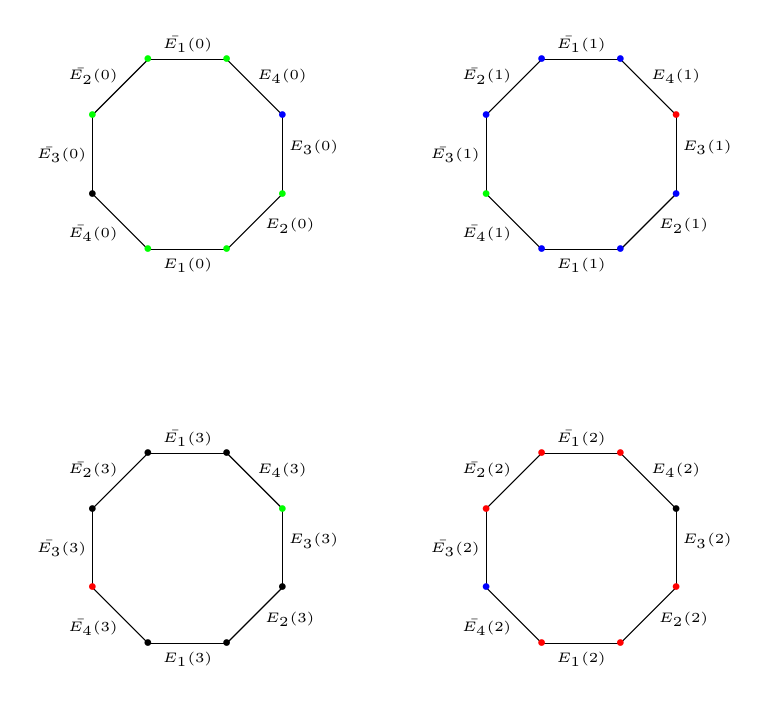
\begin{tikzpicture}[scale=1]
\draw (0,-5)--(1,-5);
\draw (1,-5)--(1.707,-4.293);
\draw (1.707,-4.293)--(1.707,-3.293);
\draw  (1.707,-3.293)--(1,-2.586);
\draw (0, -2.586)--(1,-2.586);
\draw (0,-2.586)--(-0.707,-3.293);
\draw (-0.707,-3.293)--(-0.707,-4.293);
\draw (-0.707,-4.293)--(0,-5);

\draw (0.5,-5.2) node{\tiny$E_1(0)$};
\draw (1.8,-4.7) node{\tiny$E_2(0)$};
\draw (2.1,-3.7) node{\tiny$E_3(0)$};
\draw (1.7,-2.8) node{\tiny$E_4(0)$};
\draw (0.5,-2.4) node{\tiny$\bar{E_1}(0)$};
\draw (-0.7,-2.8) node{\tiny$\bar{E_2}(0)$};
\draw (-1.1,-3.8) node{\tiny$\bar{E_3}(0)$};
\draw (-0.7,-4.8) node{\tiny$\bar{E_4}(0)$};

\draw[green] (0,-5) node{\tiny$\bullet$};
\draw[green] (1,-5) node{\tiny$\bullet$};
\draw[green] (1.707,-4.293) node{\tiny$\bullet$};
\draw[blue] (1.707,-3.293) node{\tiny$\bullet$};
\draw[green] (1,-2.586) node{\tiny$\bullet$};
\draw[green] (0,-2.586) node{\tiny$\bullet$};
\draw[green] (-0.707,-3.293) node{\tiny$\bullet$};
\draw (-0.707,-4.293) node{\tiny$\bullet$};


\draw (5,-5)--(6,-5);
\draw (6,-5)--(6.707,-4.293);
\draw (6.707,-4.293)--(6.707,-3.293);
\draw  (6.707,-3.293)--(6,-2.586);
\draw (5, -2.586)--(6,-2.586);
\draw (5,-2.586)--(4.293,-3.293);
\draw (4.293,-3.293)--(4.293,-4.293);
\draw (4.293,-4.293)--(5,-5);

\draw (5.5,-5.2) node{\tiny$E_1(1)$};
\draw (6.8,-4.7) node{\tiny$E_2(1)$};
\draw (7.1,-3.7) node{\tiny$E_3(1)$};
\draw (6.7,-2.8) node{\tiny$E_4(1)$};
\draw (5.5,-2.4) node{\tiny$\bar{E_1}(1)$};
\draw (4.3,-2.8) node{\tiny$\bar{E_2}(1)$};
\draw (3.9,-3.8) node{\tiny$\bar{E_3}(1)$};
\draw (4.3,-4.8) node{\tiny$\bar{E_4}(1)$};

\draw[blue] (5,-5) node{\tiny$\bullet$};
\draw[blue] (6,-5) node{\tiny$\bullet$};
\draw[blue] (6.707,-4.293) node{\tiny$\bullet$};
\draw[red] (6.707,-3.293) node{\tiny$\bullet$};
\draw[blue] (6,-2.586) node{\tiny$\bullet$};
\draw[blue] (5,-2.586) node{\tiny$\bullet$};
\draw[blue] (4.293,-3.293) node{\tiny$\bullet$};
\draw[green] (4.293,-4.293) node{\tiny$\bullet$};


\draw (5,-10)--(6,-10);
\draw (6,-10)--(6.707,-9.293);
\draw (6.707,-9.293)--(6.707,-8.293);
\draw  (6.707,-8.293)--(6,-7.586);
\draw (5, -7.586)--(6,-7.586);
\draw (5,-7.586)--(4.293,-8.293);
\draw (4.293,-8.293)--(4.293,-9.293);
\draw (4.293,-9.293)--(5,-10);

\draw (5.5,-10.2) node{\tiny$E_1(2)$};
\draw (6.8,-9.7) node{\tiny$E_2(2)$};
\draw (7.1,-8.7) node{\tiny$E_3(2)$};
\draw (6.7,-7.8) node{\tiny$E_4(2)$};
\draw (5.5,-7.4) node{\tiny$\bar{E_1}(2)$};
\draw (4.3,-7.8) node{\tiny$\bar{E_2}(2)$};
\draw (3.9,-8.8) node{\tiny$\bar{E_3}(2)$};
\draw (4.3,-9.8) node{\tiny$\bar{E_4}(2)$};

\draw[red] (5,-10) node{\tiny$\bullet$};
\draw[red] (6,-10) node{\tiny$\bullet$};
\draw[red] (6.707,-9.293) node{\tiny$\bullet$};
\draw (6.707,-8.293) node{\tiny$\bullet$};
\draw[red] (6,-7.586) node{\tiny$\bullet$};
\draw[red] (5,-7.586) node{\tiny$\bullet$};
\draw[red] (4.293,-8.293) node{\tiny$\bullet$};
\draw[blue] (4.293,-9.293) node{\tiny$\bullet$};


\draw (0,-10)--(1,-10);
\draw (1,-10)--(1.707,-9.293);
\draw (1.707,-9.293)--(1.707,-8.293);
\draw  (1.707,-8.293)--(1,-7.586);
\draw (0, -7.586)--(1,-7.586);
\draw (0,-7.586)--(-0.707,-8.293);
\draw (-0.707,-8.293)--(-0.707,-9.293);
\draw (-0.707,-9.293)--(0,-10);

\draw (0.5,-10.2) node{\tiny$E_1(3)$};
\draw (1.8,-9.7) node{\tiny$E_2(3)$};
\draw (2.1,-8.7) node{\tiny$E_3(3)$};
\draw (1.7,-7.8) node{\tiny$E_4(3)$};
\draw (0.5,-7.4) node{\tiny$\bar{E_1}(3)$};
\draw (-0.7,-7.8) node{\tiny$\bar{E_2}(3)$};
\draw (-1.1,-8.8) node{\tiny$\bar{E_3}(3)$};
\draw (-0.7,-9.8) node{\tiny$\bar{E_4}(3)$};

\draw (0,-10) node{\tiny$\bullet$};
\draw (1,-10) node{\tiny$\bullet$};
\draw (1.707,-9.293) node{\tiny$\bullet$};
\draw[green] (1.707,-8.293) node{\tiny$\bullet$};
\draw (1,-7.586) node{\tiny$\bullet$};
\draw (0,-7.586) node{\tiny$\bullet$};
\draw (-0.707,-8.293) node{\tiny$\bullet$};
\draw[red] (-0.707,-9.293) node{\tiny$\bullet$};

\end{tikzpicture}
\caption{Translation surface for $G_{4,2}^\prime$.}
\label{figure17}
\end{center}
\end{figure}
Also, in this case we  consider the permutation $\sigma$ = ($0$ $1$ $2$ \dots $n-1$) from $S_n$. Similarly to case $1$, we take $n$ numbers of regular $4m$ gons denoted by $P_0$, $P_1$, $P_2$, \dots, $P_{n-1}$. Label the sides of $P_i$ as $E_1(i), E_2(i), \dots, E_{2m}(i), \bar{E_1}(i), \bar{E_2}(i), 
\dots \bar{E}_{2m}(i)$ such that $E_k(i)$ is parallel to $\bar{E_k}(i)$, $1\leq k\leq m$ for each $i\in \{0,1,2 \dots, n-1\}$. Here, we form the translation surface as follows:

For a fixed $i\in \{0,1,2 \dots, n-1\}$ we identify the sides $E_k(i)$ and $\bar{E}_k(i)$  for $1\le k\le m$ and the sides $E_k(i)$ and $\bar{E}_k(\sigma(i))$ for $m+1\le k\le 2m$ via translation. So, we get a translation surface $S$ from this with $n$ number of singular points (or marked points) and each side of $P_i$'s is systolic connection of S. Therefore, $G$ admits cellular-systolic embedding on $S$. In Figure \ref{figure17}, a translation surface is explicitly constructed for $G_{4,2}^\prime$. 

The genus of the translation surface for both the cases is $\left[n(m-1)+1\right]$.

Therefore, from both the cases we conclude that any $G\in \mathcal{P} \sqcup \mathcal{Q}$ admits cellular-systolic embedding on a translation surface.

\end{proof}

\end{document}
